\documentclass[12pt]{article}
\usepackage[letterpaper,margin=.65in,headheight=18pt,headsep=18pt,footskip=25pt]{geometry}
\usepackage[T1]{fontenc}\usepackage{helvet}\renewcommand{\familydefault}{\sfdefault}
\usepackage{tikz,array,fancyhdr}\usetikzlibrary{arrows.meta,decorations.pathreplacing}
\pagestyle{fancy}\fancyhf{}\renewcommand{\headrulewidth}{0pt}
\fancyhead[L]{\small Week 32 / Square recipes encore / Grades 2--5}
\fancyfoot[L]{\scriptsize Bellingham Math Circle / Week 32 / W32-BON-v1}\fancyfoot[R]{\scriptsize\thepage}
\setlength{\parindent}{0pt}\setlength{\parskip}{9pt}
\newcommand{\problem}[2]{\par\textbf{Problem #1:} #2\par}
\newcommand{\board}[3]{\begin{tikzpicture}[x=1cm,y=1cm]\draw[step=1,black!20,very thin] (0,0) grid (#1,#2);\draw[line width=.8pt] (0,0) rectangle (#1,#2);\node[anchor=north] at (#1/2,-.25){#3};\end{tikzpicture}}
\newcommand{\workspace}[1]{\begin{tikzpicture}[x=1cm,y=1cm]\draw[step=1,black!20,very thin] (0,0) grid (8,4);\draw[dashed,black!50] (0,0) rectangle (8,4);\node[anchor=north] at (4,-.25){recipe: #1};\end{tikzpicture}}
\begin{document}
Squares must fill the rectangle, with no gaps, overlaps, or overhang. All edges stay on grid lines. The biggest-square rule removes the largest square from one end of the remaining rectangle, then repeats.
\problem{1}{For each rectangle, use the biggest-square rule on the left board. Tile the right board with as few squares as you can, using any whole-number sizes.}
\begin{center}\begin{tabular}{cc}
\board{6}{5}{biggest-square rule}&\board{6}{5}{fewest squares}\\[8mm]
\board{4}{3}{biggest-square rule}&\board{4}{3}{fewest squares}
\end{tabular}\end{center}
\vspace{8mm}
\problem{2}{What is the fewest number of squares for the $6\times5$ rectangle? Explain why a tiling with fewer squares cannot fit.}
\vspace{3cm}
\newpage
\problem{3}{Use only $2\times2$ and $3\times3$ squares. Which rectangles can you fill? Draw a tiling for each possible one. Explain why the others cannot be filled.}
\begin{center}\begin{tabular}{cc}
\board{5}{5}{$5\times5$}&\board{6}{5}{$6\times5$}\\[8mm]
\multicolumn{2}{c}{\board{7}{5}{$7\times5$}}
\end{tabular}\end{center}
\vspace{4cm}
\newpage
A recipe lists how many consecutive squares of each size the biggest-square rule removes, from largest size to smallest. The sizes are left out.
\begin{center}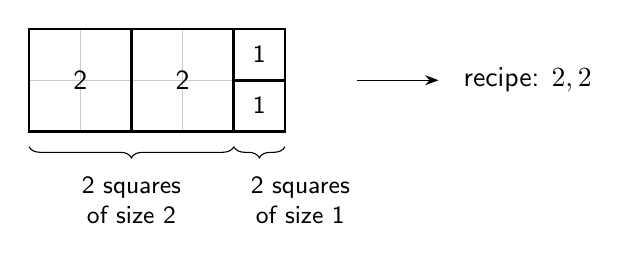
\begin{tikzpicture}[x=.65cm,y=.65cm,>=Stealth]
\draw[step=1,black!20,very thin] (0,0) grid (5,2);
\draw[line width=1pt] (0,0) rectangle (2,2);\draw[line width=1pt] (2,0) rectangle (4,2);
\draw[line width=1pt] (4,0) rectangle (5,1);\draw[line width=1pt] (4,1) rectangle (5,2);
\node at (1,1){2};\node at (3,1){2};\node[font=\small] at (4.5,.5){1};\node[font=\small] at (4.5,1.5){1};
\draw[decorate,decoration={brace,mirror,amplitude=4pt}] (0,-.3)--(4,-.3);
\node[anchor=north,font=\small,align=center] at (2,-.7){2 squares\\of size 2};
\draw[decorate,decoration={brace,mirror,amplitude=4pt}] (4,-.3)--(5,-.3);
\node[anchor=north,font=\small,align=center] at (5.3,-.7){2 squares\\of size 1};
\draw[->] (6.4,1)--(8,1);\node[anchor=west] at (8.3,1){recipe: $2,2$};
\end{tikzpicture}\end{center}
\problem{4}{For each recipe, draw a rectangle and its square tiling on the grid. Choose its square sizes yourself, then check it with the biggest-square rule. Can different-sized rectangles have the same recipe? You may use separate graph paper.}
\begin{center}
\workspace{$1,2$}\par\vspace{8mm}
\workspace{$2,1,2$}\par\vspace{8mm}
\workspace{$1,1,3$}
\end{center}
\vspace{1cm}
\end{document}
